%
% 1-koordinaten.tex -- Koordinaten
%
% (c) 2024 Prof Dr Andreas Müller
%
\section{Koordinaten
\label{buch:koordinaten:section:koordinaten}}
\kopfrechts{Koordinaten}
In diesem Abschnitt betrachten wir eine Punktmenge $X$, die mit
Koordinatensystemen ausgestattet werden soll.
Ohne das Koordinatensystem hat die Punktemenge keinerlei Struktur.
Um von stetigen Abbildungen zwischen solchen Mengen zu sprechen,
wird zum Beispiel ein Begriff der Nähe benötigt, mit dem die Konvergenz
von Folgen definiert werden kann.
Die Konstruktion eines Koordinatensystems ermöglicht, Punkte also
nahe beeinander zu betrachten, wenn sich ihre Koordinaten nur geringfügig
unterscheiden.

%
% Koordinatensystem
%
\subsection{Koordinatensystem}
%
% fig-koordinaten.tex
%
% (c) 2024 Prof Dr Andreas Müller
%
\begin{figure}
\centering
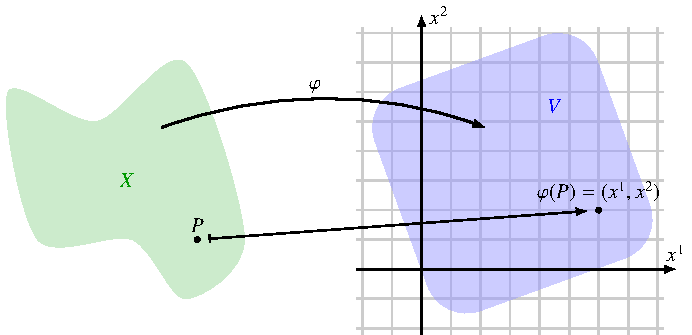
\includegraphics{chapters/020-koordinaten/images/koordinaten.pdf}
\caption{Ein Koordinatensystem auf der Punktmenge $X$ ist eine Abbildung 
$\varphi$ in den Koordinatenraum $V$, der eine Teilmenge von
$\mathbb{R}^n$ ist.
\label{buch:koordinaten:koordinaten:fig:koordinaten}}
\end{figure}
%
Ein $n$-dimensionales Koordinatensystem auf $X$ ordnet jedem Punkt 
ein $n$-Tupel von Koordinaten zu.
Aus erst später verständlichen Gründen bezeichnen wir die Koordinaten
mit hochgestellten Indizes, wir schreiben also $x^1,\dots,x^n$.
\index{Koordinaten}%
Eine Verwechslungsgefahr mit Exponenten besteht normalerweise nicht.
Falls die $k$-te Potenz der Koordinate $x^1$ berechnet werden soll, 
wird dies mit Klammern als $(x^i)^k$ geschrieben.
Ein Koordinatensystem ist also eine Abbildung
\[
\varphi
\colon
X\to \mathbb{R}^n
:
P \mapsto (x^1,\dots,x^n),
\]
wie sie in Abbildung~\ref{buch:koordinaten:koordinaten:fig:koordinaten}
dargestellt ist.
Jede einzelne Koordinate kann als Funktion $P\mapsto x^i(P)$ mit
reellen Werten betrachtet werden.

\begin{beispiel}
\label{buch:koordinaten:koordinaten:beispiel:kartpolar}
%
% fit-kartpolar.tex%
%
% (c) 2024 Prof Dr Andreas Müller
%
\begin{figure}
\centering
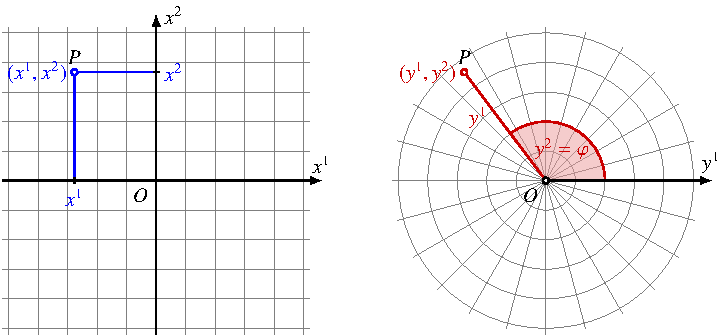
\includegraphics{chapters/020-koordinaten/images/kartpolar.pdf}
\caption{Zwei Koordinatensysteme für die Ebene:
kartesische (rechtwinklige) Koordinaten links und Polarkoordinaten
rechts.
Der gleiche Punkt $P$ wird gleichermassen durch die Koordinaten 
$(x^1,x^2)$ und $(y^1,y^2)$ beschrieben.
\label{buch:koordinaten:fig:kartpolar}}
\end{figure}

Die Punkte einer Ebene können einerseits mit dem {\em kartesischen}
Koordinatensystem mit den Koordinaten $(x^1,x^2)\in\mathbb{R}$ 
beschrieben werden und andererseits durch {\em Polarkoordinaten},
\index{Polarkoordinaten}%
\index{kartesische Koordinaten}%
die einen Punkt durch den Radius $y^1 = r$ und den Polarwinkel
\index{Polarwinkel}%
$y^2 = \varphi$ definieren (Abbildung~\ref{buch:koordinaten:fig:kartpolar}).

Die kartesischen Koordinaten können aus den Polarkoordinaten durch
\begin{equation}
\left.
\begin{aligned}
x^1 &= y^1\cos y^2 \\
x^2 &= y^1\sin y^2
\end{aligned}
\qquad
\right\}
\label{buch:koordinaten:koordinaten:eqn:polarkartumrechnung}
\end{equation}
berechnet werden.
\end{beispiel}

\begin{beispiel}
\label{buch:koordinaten:koordinaten:beispiel:kartkugel}
%
% fig-kartkugel.tex
%
% (c) 2024 Prof Dr Andreas Müller
%
\begin{figure}
\centering
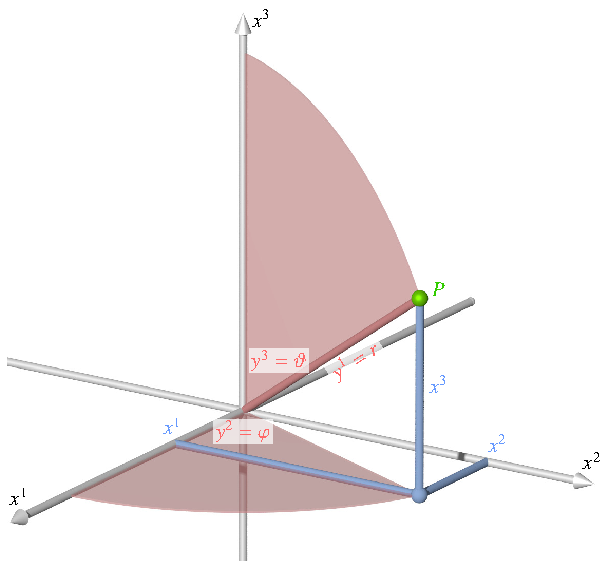
\includegraphics{chapters/020-koordinaten/images/kartkugel.pdf}
\caption{Kartesische Koordinaten ({\color{blue}blau}) und Kugelkoordinaten
({\color{darkred}rot}) für einen Punkt $P$ des dreidmensionalen Raumes.
\label{buch:koordinaten:koordinaten:fig:kartkugel}}
\end{figure}

Der dreidimensionale Raum kann sowohl durch {\em kartesische}
Koordinatentripel $(x^1,x^2,x^3)$ wie auch durch {\em Kugelkoordinaten}
\index{Kugelkoordinaten}%
beschrieben werden.
In Kugelkoordinaten ist ein Punkt durch die Entfernung $r=y^1$ vom
Nullpunkt, den Polarwinkel $y^2=\varphi$ seiner Projektion in die 
\index{Nullpunkt}%
$x^1$-$x^2$-Ebene und den Winkel $\vartheta$ zwischen der positiven
$x^3$-Achse und der Geraden durch Nullpunkt $O$ und den Punkt gegeben
(Abbildung~\ref{buch:koordinaten:koordinaten:fig:kartkugel}).
Die Umrechnung von Kugelkoordinaten in kartesische Koordinaten
\index{Kugelkoordinate}%
erfolgt mit
\begin{equation}
\left.
\begin{aligned}
x^1
&=
y^1 \cos y^2 \cos y^3 \\
x^2
&=
y^1 \sin y^2 \cos y^3 \\
x^3
&=
y^2 \cos y^3.
\end{aligned}
\qquad\right\}
\label{buch:koordinaten:koordinaten:eqn:kugelkartumrechnung}
\end{equation}
Man beachte, dass Punkte auf der $x^3$-Achse $y^3=0$ oder
$y^3=\pi$ und beliebigen Winkel $y^2\in\mathbb{R}$ haben.
Ohne zusätzliche Einschränkungen haben die Punkte auf der
$x^3$-Achse keine eindeutigen Kugelkoordinaten.
\end{beispiel}

Um die Struktur des Koordinatenraumes $\mathbb{R}^n$ auf die Menge
$X$ zu übertragen, müssen die Koordinatenabbildungen weiter eingeschränkt
werden.
Zunächst muss die Koordinatenabbildung bijektiv sein.
Dies bedeutet, dass jeder Punkt durch genau ein Koordinaten-$n$-Tupel
beschrieben wird.
Diese Bedingung ist in beiden Beispielen nicht erfüllt, da Tupel,
deren $y^2=\varphi$-Koordinaten sich um $2\pi$ unterscheiden, den
gleichen Punkt beschreiben.
Sie ist aber für genügend kleine Teilmengen des Raumes erfüllt.

Tatsächlich kann man nicht erwarten, zum Beispiel die Oberfläche einer
Kugel oder eines Torus in ihrer Gesamtheit eineindeutig auf Ebene
abzubilden.
Die Definition eines Koordinatensystems ist vorerst also nur geeignet,
eine Punktmenge lokal zu beschreiben.
Für eine globale Beschreibung wird es notwendig sein, verschiedene
Koordinatensysteme, die auf Teilen einer Menge definiert sind, zu
einem grösseren Ganzen zusammenzufügen.

Ausserdem muss die Menge $V=\varphi(X)$ der möglichen Koordinaten-$n$-Tupel
eine offene Menge in $\mathbb{R}^n$ sein.
Auch diese Bedingung ist in den Beispielen nicht erfüllt.
Die $y^1=r$-Koordinate nimmt alle Werte in
\[
\mathbb{R}_{\ge 0}
=
[0,\infty)
=
\{
y^1\in\mathbb{R}
\mid
y^1\ge 0
\}.
\]
\index{R@$\mathbb{R}_{\ge 0}$}%
Dies ist keine offene Menge, da die Punkte $(0,y^2)$ bzw.~$(0,y^2,y^3)$
ein Randpunkt des Wertebereichs der $y$-Koordinaten ist.
\index{offene Menge}%
\index{Randpunkt}%
Bei Kugelkoordinaten nimmt die Koordinate $y^3$ Werte im
abgeschlossenen Interval $[0,\pi]$ an, was zu weiteren Randpunkten
des Wertebereichs führen.

% XXX Beispiel zur Notwendigkeit der letzten Bedingung zeigen

%
% Koordinatenwechsel
%
\subsection{Koordinatenwechsel
\label{buch:koordinaten:koordinaten:subsection:koordinatenwechsel}}
In den Beispielen
\ref{buch:koordinaten:koordinaten:beispiel:kartpolar}
und
\ref{buch:koordinaten:koordinaten:beispiel:kartkugel}
wurden bereits Umrechnungsformeln zwischen den dort dargestellten
Koordinatensystemen ermittelt.
Seien etwas allgemeiner zwei Koordinatensysteme $x^1,\dots,x^n$
und $y^1,\dots,y^n$ auf der Punktmenge $X$ gegeben.
Sei $U$ die Menge der Koordinaten-$n$-Tupel, die Punkte von $X$
in den $x^i$-Koordinaten beschreiben, also die Bildmenge der
Koordinatenabbildung $\varphi$.
Dann ist die Umkehrabbildung $\varphi^{-1}$ auf $U$ definiert.

Sei weiter $\psi$ die Koordinatenabbildung für die $y^i$-Koordinaten
und $V$ der zugehörige Wertebereich.
Die Zusammensetzung
\[
\psi
\circ
\varphi^{-1}
\colon
U\to V\subset\mathbb{R}^n
:
(x^1,\dots,x^n)
\mapsto
(y^1,\dots,y^n)
\]
ist die Koordinatenumrechnung vom $x^i$-Koordinatensystem in
das $y^i$-Koordinatensystem, eine Abbildung von $U$ in $V\subset\mathbb{R}^n$.

% XXX Koordinatenwechsel-Abbildung

Die Koordinatenwechsel-Abbildung ist umkehrbar, da sowohl $\varphi$
als auch $\psi$ umkehrbar sind.
\index{Koordinatenwechsel}
Die Umkehrabbildung ist die Abbildung
\[
(\psi\circ\varphi^{-1})^{-1}
=
\varphi\circ\psi^{-1}
\colon
V\to W \subset \mathbb{R}^n.
\]

%
% Stetigkeit
%
\subsubsection{Stetigkeit}
Die Koordinatenabbildungen $\varphi$ ermöglicht, auf der Menge
$X$ zu definieren, was eine konvergente Folge ist.
Die Punkte $P_k\in X$ konvergieren genau dann gegen den Punkt $P$,
wenn die Bildpunkte $\varphi(P_k)$ in $U$ gegen $\varphi(P)$
konvergieren.

Eine weitere Koordinatenabbildung $\psi\colon X\to V$ definiert einen
weiteren Begriff der Konvergenz von Punktfolgen in $X$.
Die Eigenschaft einer Folge, zu konvergieren, sollte nicht davon 
abhängig sein, in welchen Koordinaten der Grenzwert berechnet
werden soll.
Für jedes Koordinatensystem sollte sich der gleiche Begriff der
Konvergenz von Folgen ergeben.
Dies schränkt die Menge der zulässigen Koordinatensysteme ein.

Zwei Koordinatensysteme $\varphi$ und $\psi$ führen auf den gleichen
Konvergenzbegriff, wenn für jede Folge $P_k\in X$ die Folgen
\[
x_k=\varphi(P_k)\in V
\qquad\text{und}\qquad
y_k=\psi(P_k)\in W
\]
beide konvergent oder beide nicht konvergent sind.
Dies trifft genau dann zu, wenn die Koordinatenwechselabbildungen
$\psi\circ\varphi^{-1}$ in jedem Punkt stetig sind.

Die Konvergenz einer Folge in $\mathbb{R}^n$ wird durch das Verhalten
der Entfernung
\[
d(P,Q)
=
|x(P)-x(Q)|
\]
von Punkten bestimmt.
Die Funktion $d$ heisst auch die vom Koordinatensystem induzierte 
{\em Metrik}.
\index{Metrik}%
Eine Folge $P_k$ konvergiert gegen $P$, wenn es für jedes $\varepsilon>0$
eine Zahl $N$ gibt derart, dass der Abstand $d(P,P_k)<\varepsilon$, wenn
$k>N$ ist.
Der Begriff des Abstandes von Punkten lässt sich mit der Koordinatenabbildung
nicht auf die Menge $X$ übertragen, da die Abstände je nach Koordinatensystem
verschieden sein können.
Dies ist aber auch nicht nötig, denn Konvergenz verlangt nur, dass genügend
kleine Abstände in einem Koordinatensystem auch genügend klein sind in jedem
anderen Koordinatensystem.
Die Koordinatenwechselabbildung $\psi\circ\varphi^{-1}$  muss daher die
Bedingung erfüllen, dass es für jedes $\varepsilon>0$ ein $\delta>0$ gibt,
dass 
\[
|y(P)-y(Q)| < \varepsilon
\]
für alle Paare von Punkten $P$ und $Q$ mit $|x(P)-x(Q)| < \delta$
gilt.
Dies ist aber die Definition einer stetigen Abbildung.

\begin{definition}[offene Menge in $X$]
\label{buch:koordinaten:koordinaten:definition:offenemenge}
Eine Menge $U\subset X$ heisst eine {\em offene Menge}, wenn es für jeden Punkt
\index{offene Menge}%
\index{Menge, offen}%
$P\in X$ und für jedes Koordinatensystem $\varphi\colon X\to V$
ein $\varepsilon >0$ gibt derart, dass die Menge
\[
U_{P,\varphi}
=
\varphi^{-1}\bigl(
\{
x\in V
\mid
|x-\varphi(P)|<\varepsilon
\}
\bigr)
\]
in $U$ enthalten ist: $U_{P,\varphi}\subset U$.
\end{definition}

Die Definition transportiert die Idee einer kleinen Umgebung
eines Punktes mithilfe der Koordinatenabbildung von der Bildmenge
$V\subset \mathbb{R}^n$ auf die Menge $X$.
Damit sich daraus ein konsistenter Begriff der kleinen Umgebung 
ergibt, müssen verschiedene Koordinatensysteme die gleichen
kleinen Umgebungen erzeugen.
Dies wird durch die folgende Definition sichergestellt.

\begin{definition}[stetige Struktur]
\label{buch:koordinaten:koordinaten:definition:stetigestruktur}
\index{stetige Struktur}%
\index{Struktur!stetig}%
Eine {\em stetige Struktur} auf der Punktemenge $X$ ist eine mit
der Indexmenge $I$ indizierte Familie
\[
\varphi_\alpha\colon X\to V_\alpha \subset \mathbb{R}^n,
\]
$\alpha\in I$,
von Koordinatensystemen auf der Menge $X$ derart, dass die
Koordinatenwechselabbildungen
\[
\varphi_{\beta}\circ\varphi_\alpha^{-1}
\colon
V_\alpha \to V_\beta
\]
stetige Abbildungen für alle $\alpha,\beta\in I$ sind.
\end{definition}

Mit jedem Koordinatenwechsel ist auch die Umkehrabbildung ein
Koordinantenwechsel.
Die Koordinatenwechsel sind also alle umkehrbare stetige Abbildungen,
oder {\em Homöomorphismen}.
\index{Homoomorphismus@Homöomorphismus}%

Will man ein neues Koordinatensystem auf $X$ verwenden, muss es so
gewählt werden, dass es mit allen bereits verwendeten Koordinatensystemen
verträglich ist.
Die Koordinatenwechsel von und zum neuen Koordinatensystem müssen
alle stetig sein.

%
% Stetige Funktionen auf X
%
\subsubsection{Stetige Funktionen auf $X$}
Sei jetzt $f\colon X\to\mathbb{R}$ eine reellwertige Funktion.
Ohne ein Koordinatensystem ist nicht klar, was es heissen soll, dass die
Funktion $f$ stetig ist.
Mit Hilfe eines Koordinatensystems $\varphi\colon X\to V$ kann man die
Funktion $f$ jetzt auch in Koordinaten schreiben.
Dazu bildet man die Funktion
\[
f_\varphi
=
f\circ \varphi^{-1}
\colon
V
\to
\mathbb{R}
:
(x^1,\dots,x^n)
\mapsto
f(\varphi^{-1}(x^1,\dots,x^n))
=
f(x^1,\dots,x^n).
\]
Eine Funktion $f$ heisst stetig, wenn die in $x$-Koordinaten geschriebene
Funktion $f(x^1,\dots,x^n)$ eine stetige Funktion ist.
Wählt man ein anderes Koordinatensystem $\psi\colon X\to W$ einer
stetigen Struktur auf $X$, dann ist der Koordinatenwechsel
$\varphi\circ\psi^{-1}$ ein Homöomorphismus, insbesondere ist 
\[
f_\psi
=
f\circ\psi^{-1}
=
\underbrace{f\circ\varphi^{-1}}_{\displaystyle f_\varphi\mathstrut}
\circ
\underbrace{\varphi\circ\psi^{-1}}_{\displaystyle
\hbox to6pt{\rlap{\text{Koordinatenwechsel\strut}}\hfill}}
\colon
W\to \mathbb{R}
\]
genau dann stetig, wenn auch $f_\varphi$ stetig ist.
Eine stetige Struktur auf $X$ ermöglicht also insbesondere auch,
auf konsistente Weise über Stetigkeit von rellwertigen Funktionen
auf $X$ zu sprechen.

%
% Differenzierbarkeit
%
\subsubsection{Differenzierbarkeit}
Für eine beliebige Punktmenge $X$ ist es im Allgemeinen nicht sinnvoll,
von differenzierbaren Funktionen zu sprechen.
\index{differenzierbar}%
Die Existenz der Ableitung $f'(x_0)$ einer Funktion im Punkt $x_0$
basiert darauf, dass es eine lineare Ersatzfunktion
\index{lineare Ersatzfunktion}%
\begin{equation}
f(x) = f(x_0) + f'(x_0)\cdot (x-x_0)+o(x-x_0)
\label{buch:koordinaten:koordinaten:eqn:linersatz}
\end{equation}
gibt.
Die Notation $o(t)$ bezeichnet eine Funktion mit der Eigenschaft
\[
\lim_{t\to 0} \frac{o(t)}{t}=0
\]
(Lambert-$o$-Notation).
\index{Lambert-o-Notation@Lambert-$o$-Notation}%
\index{o-Notation@$o$-Notation}%
Die Darstellung~\eqref{buch:koordinaten:koordinaten:eqn:linersatz}
ist nur sinnvoll, wenn der Definitions- wie auch der Wertebereich
Teilmengen von $\mathbb{R}$ sind.

Eine Funktion $f\colon X\to \mathbb{R}$ kann in einem Koordinatensystem
$\varphi\colon X\to V\subset\mathbb{R}^n$ als Funktion
\[
f_\varphi
\colon
V\to\mathbb{R}
:
(x^1,\dots,x^n)
\mapsto
f\circ\varphi^{-1}(x^1,\dots,x^n)
\]
der Koordinaten $x^i$ geschrieben werden.
Damit ist die Voraussetzung geschaffen, von den Ableitungen von $f$
nach jeder beliebigen Koordinate zu sprechen.
Die {\em partielle Ableitung} von $f$ nach der Koordinaten $x^i$ im
Koordinatensystem $\varphi$ ist
\begin{equation}
\frac{\partial f}{\partial x^i}
=
\frac{\partial f_\varphi}{\partial x^1}(x^1,\dots,x^n)
=
\lim_{h\to 0}
\frac{f_\varphi(x^1,\dots,x^i+h,\dots, x^n)-f(x^1,\dots,x^n)}{h}.
\label{buch:koordinaten:koordinaten:eqn:partabl}
\end{equation}
Bei der Ableitung werden alle Koordinaten ausser der Koordinaten $x^i$
konstant gehalten.

Der Ausdruck~\eqref{buch:koordinaten:koordinaten:eqn:partabl} ist ganz
explizit von der Wahl des Koordinatensystems abhängig.
Sei $\psi\colon X\to W$ ein weiteres Koordinatensystem, dann lassen sich
die Koordinaten $x^i$ des Koordinatensystems $\varphi$ in die 
Koordinaten $y^k$ des Koordinatensystems $\psi$ umrechnen.
Die Koordinate $y^k$ ist eine reellwertige Funktion auf $X$, wir
können daher auch die partiellen Ableitungen
\[
\frac{\partial y^k}{\partial x^i}(x^1,\dots,x^n)
\]
bilden.
Aus der Kettenregel können jetzt die partiellen Ableitung bezüglich
\index{Kettenregel}%
der Variablen $y^k$ durch die partiellen Ableitungen bezüglich der
Variablen $x^i$ als
\begin{align*}
\frac{\partial}{\partial x^i}
(f\circ\psi^{-1})\circ (\psi\circ\varphi^{-1})(x^1,\dots,x^n)
&=
\sum_{k=1}^n
\frac{\partial f\circ\psi^{-1}}{\partial y^k}(y^1,\dots,y^n)
\cdot
\frac{\partial y^k}{\partial x^i}(x^1,\dots,x^n)
\end{align*}
ausgedrückt werden.

\begin{definition}[Jacobi-Matrix]
Die Matrix
\[
J
=
\frac{\partial(y^1,\dots,y^n)}{\partial(x^1,\dots,x^n)}
=
\bgroup
\renewcommand\arraystretch{1.8}
\begin{pmatrix}
\displaystyle\frac{\partial y^1}{\partial x^1}&\dots&\displaystyle\frac{\partial y^1}{\partial x^n}\\
\vdots&\ddots&\vdots\\[-2pt]
\displaystyle\frac{\partial y^n}{\partial x^1}&\dots&\displaystyle\frac{\partial y^n}{\partial x^n}\\
\end{pmatrix}
\egroup
\]
mit den Matrixeinträgen
\[
J_{ki}
=
\frac{\partial y^k}{\partial x^i}(x^1,\dots,x^n)
\]
heisst die {\em Jacobi-Matrix} der Funktionen $y^k(x_1,\dots,x_n)$,
$k=1,\dots,n$.
\index{Jacobi-Matrix}%
\index{J}
\end{definition}

Die Umrechnung der partiellen Ableitungen zwischen verschiedenen
Koordinatensystemen erfolgt also mit Hilfe der Jacobi-Matrix der
Koordinatentransformation.

\begin{definition}
Ein Koordinatenwechsel $\psi\circ\varphi^{-1}$ heisst
\index{Koordinatenwechsel}%
{\em stetig differenzierbar}, wenn die Jacobi-Matrix $J$
stetig ist.
\end{definition}

Die Eigenschaft der Differenzierbarkeit einer Funktion sollte wie
im Falle der Stetigkeit nicht von der Wahl eines Koordinatensystems
abhängen.
Das kann nur funktionieren, wenn die Umrechnung zwischen verschiedenen
Koordinatensystemen immer möglich ist.
Dazu muss die Jacobi-Matrix in jedem Punkt des Koordinatensystems
definiert sein.
Dies schränkt die Wahl der zulässigen Koordinatensysteme weiter ein.

\begin{definition}[differenzierbare Struktur]
\label{buch:koordinaten:koordinaten:definition:diffbareestruktur}
Eine {\em differenzierbare Struktur} auf $X$ ist eine stetige Struktur,
\index{differenzierbare Struktur}%
\index{Struktur!differenzierbar}%
deren Koordinatenwechsel stetig differenzierbar sind.
\end{definition}

